

\section{Fitting a single bivariate normal to forward and side scatter}


%% Gating
% Scatter plots
\begin{figure}[ht]
%\begin{center}
    \begin{subfigure}[b]{.5\textwidth}
        \centering
        %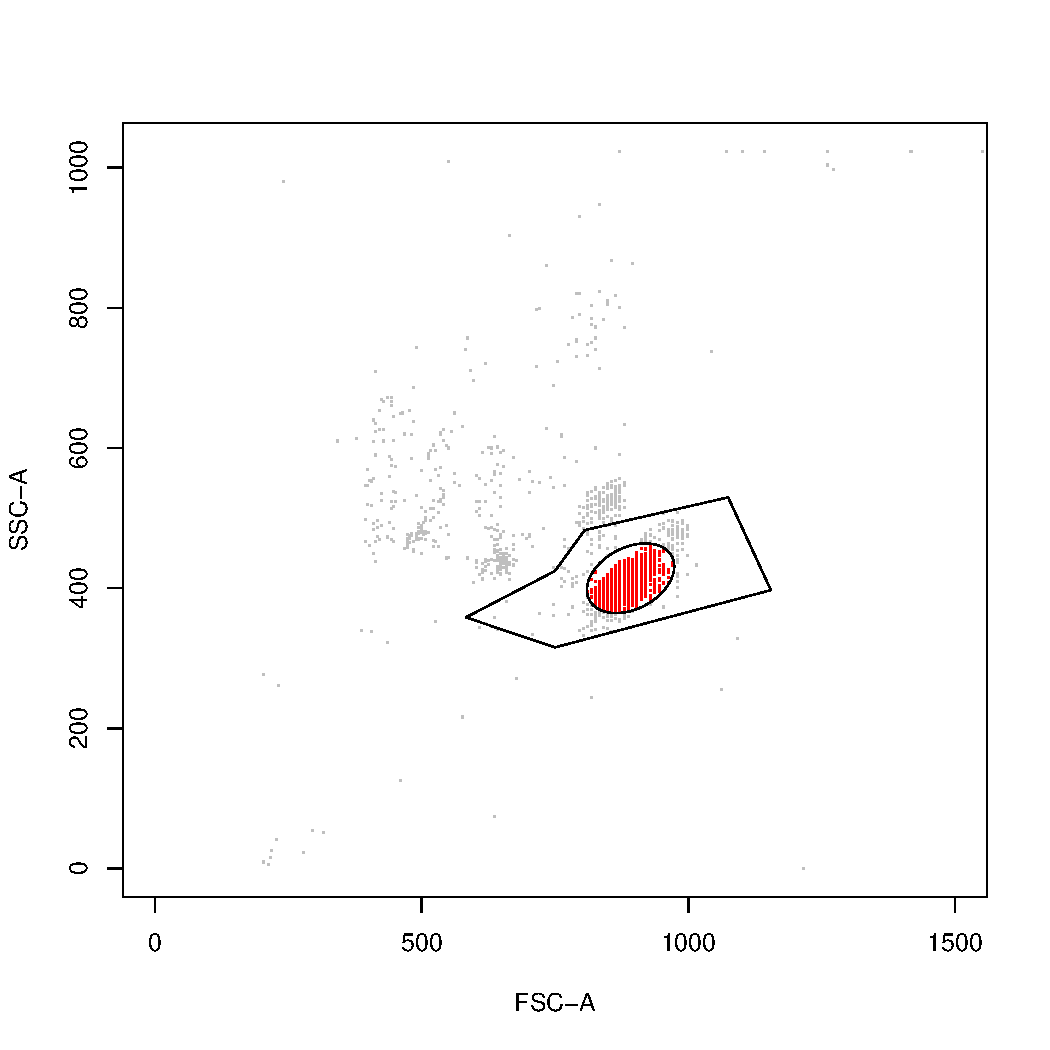
\includegraphics[scale=.5]{IL2RA/figures/Beads/manual-flowclust-scatter-gate-cad57.pdf} 
        \caption{Manual and FlowClust gating on scatter.}
    \end{subfigure}
    ~
    \begin{subfigure}[b]{.5\textwidth}
        \centering
        %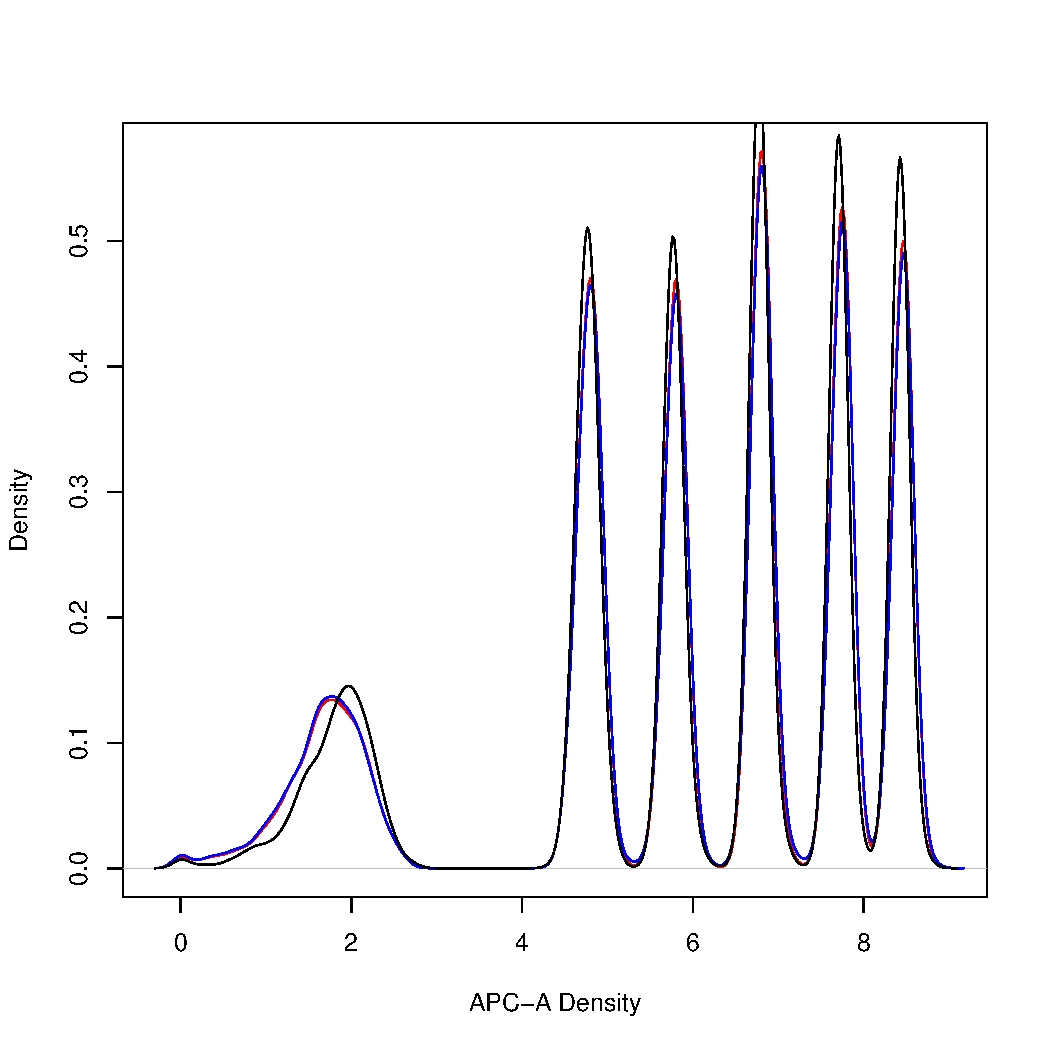
\includegraphics[scale=.5]{IL2RA/figures/Beads/manual-flowclust-apc-cad57.pdf} 
        \caption{density of $log$ APC after applying scatter gate.}
    \end{subfigure}
%\end{center}
\caption{ \label{figure:bead-gate}
  In Figure a), the gate applied by FlowClust (in red) is a subset of the gate applied through manual gating (in blue).
In Figure b) we notice that the effect of the scatter gating on the APC channel is to reduce the intensity of the first peak (the blank beads) and slightly increase the intensity of the other peaks.
Overall both manual and FlowClust gating seem to yield very similar distributions. }
\end{figure}



I first gated on both the forward and side scatter using \texttt{FlowClust} \citep{Lo:2008it}
to distinguish single beads from groups of beads which might go through the flow cytometer clumped together (Figure~\ref{figure:bead-gate}).
FlowClust proceeds by doing a Box-Cox transform to normalise the data, then fits a mixture of Student t-distributions
using the EM algorithm \citep{Dempster:1977ul}. In this case, there is a single populations as all beads are the same size.
%(Appendix~\ref{EM}).
%To filter out the predominant population of single beads, I fitted a single bivariate Student t-distribution on the two scatter dimensions (side and forward)\footnote{In this case, given we know that the number of clusters $K=1$ an even simpler way would be to use a single bivariate Gaussian.}.


